\documentclass{llncs}

\usepackage[T1]{fontenc}
\usepackage{amsmath,amssymb,mathtools}
\usepackage{graphicx}
\usepackage{booktabs}
\usepackage{tikz}
\usetikzlibrary{arrows.meta,positioning}
\usepackage{enumitem}
\usepackage{microtype}
\usepackage{url}

\newcommand{\clip}{\Pi}
\newcommand{\R}{\mathbb{R}}
\newcommand{\GA}{G_A}
\newcommand{\GX}{G_X}
\newcommand{\eps}{\varepsilon}
\newcommand{\T}{T_{[0,1]}}
\newcommand{\poly}{\operatorname{poly}}
\DeclareMathOperator{\SOL}{SOL}

\begin{document}

\begin{center}
{\LARGE\bfseries Sign-Balanced Liquidation Clearing in DeFi Markets\par}
\end{center}
\vspace{-0.2em}

\begin{abstract}
Liquidations in DeFi lending protocols are interdependent: selling collateral moves prices, which can trigger or suppress other liquidations. We study a collateral-only liquidation model with linear price impact, in which liquidators repay debt externally and only collateral sales move market prices. Even in this conservative mechanism, clearing can be nonmonotone: when an asset sold as collateral is also used as another position's debt asset, its price decline reduces that borrower's debt burden.

We identify a sign-balance frontier. If the asset borrowing graph is bipartite, then after flipping one side of the asset prices and complementing liquidation variables on one side, the smooth clearing equations become \(y=\clip_{[0,u]}(Ay+c)\) with \(A\ge 0\). This is equivalent to a box complementarity problem with a Z-matrix and can be solved in polynomial time via a single linear program for its least element. Conversely, in the non-bipartite regime, constant-approximate clearing is PPAD-hard. The reduction uses only two liquidation primitives: a NOT gadget implementing debt-relief feedback and a truncated-SUM gadget implemented by co-writers selling the same output collateral. Thus the hardness does not rely on credit default swaps, debt-side buying pressure, or high-gain comparators. Smooth approximate clearing is in PPAD, and all-or-nothing clearing is in NP with a polynomial-time balanced case.
\keywords{DeFi liquidation \and Clearing \and PPAD \and Linear complementarity \and Z-matrices \and Financial networks}
\end{abstract}

\section{Introduction and Technical Overview}
\label{sec:intro}
DeFi lending protocols liquidate undercollateralized positions. A position has a collateral asset and a debt asset. If it becomes unhealthy, liquidators repay debt and receive collateral; at the market level, the relevant price impact is that collateral is sold. When positions are large relative to liquidity, these sales move prices, and those price movements affect the health of other positions. A clearing is a self-consistent vector of liquidations and prices: the liquidations implied by prices must be exactly the liquidations whose collateral sales generate those prices.

This paper studies the computational problem created by this feedback. We use a linear price-impact market as a first-order model of liquidation-induced price movement. This modeling choice is deliberately conservative. Liquidations only sell collateral; debts are repaid externally. There is no market buy pressure on the debt asset. Thus the nonmonotonicity we identify does not arise from an artificial assumption that liquidators buy debt in the same market. It arises from the fact that the same asset can appear as collateral in one position and as debt in another.

\paragraph{A DeFi-native negative feedback.}
Consider three assets \(A,B,C\) and three positions
\[
P_1=(A,B),\qquad P_2=(B,C),\qquad P_3=(C,A),
\]
where \((A,B)\) denotes collateral \(A\) and debt \(B\). If \(P_1\) is liquidated more aggressively, more \(A\) is sold and \(p_A\) falls. But \(A\) is the debt asset of \(P_3\), so the value of \(P_3\)'s debt falls. Thus \(P_3\) becomes healthier and may liquidate less. A liquidation can therefore rescue another borrower whose debt is denominated in the asset being sold. This effect creates an all-negative cycle of liquidation feedback; see Fig.~\ref{fig:triangle}. It is the primitive behind both our sign-balance theorem and our hardness gadgets.

\begin{figure}[t]
\centering
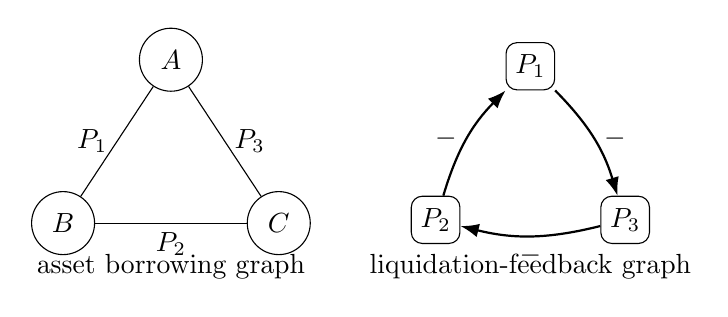
\begin{tikzpicture}[scale=0.83, asset/.style={circle,draw,minimum size=8mm}, pnode/.style={rectangle,draw,rounded corners,minimum height=6mm}, >=Latex]
  \node[asset] (A) at (0,1.55) {$A$};
  \node[asset] (B) at (-1.65,-.95) {$B$};
  \node[asset] (C) at (1.65,-.95) {$C$};
  \draw[-] (A)--node[left] {$P_1$} (B);
  \draw[-] (B)--node[below] {$P_2$} (C);
  \draw[-] (C)--node[right] {$P_3$} (A);
  \node at (0,-1.62) {asset borrowing graph};

  \node[pnode] (p1) at (5.5,1.45) {$P_1$};
  \node[pnode] (p2) at (4.05,-.9) {$P_2$};
  \node[pnode] (p3) at (6.95,-.9) {$P_3$};
  \draw[->,thick] (p1) to[bend left=14] node[right] {$-$} (p3);
  \draw[->,thick] (p3) to[bend left=14] node[below] {$-$} (p2);
  \draw[->,thick] (p2) to[bend left=14] node[left] {$-$} (p1);
  \node at (5.5,-1.62) {liquidation-feedback graph};
\end{tikzpicture}
\caption{A three-asset collateral-debt cycle. Selling an asset can lower another position's debt value, creating a negative liquidation dependency.}
\label{fig:triangle}
\end{figure}

\paragraph{Main results.}
Our positive result identifies a tractable sign-balanced regime. Let \(\GA\) be the asset borrowing graph: its vertices are assets and each position gives an edge between its collateral and debt assets.
\begin{quote}
\textbf{Balanced tractability.} If \(\GA\) is bipartite, smooth collateral-only clearing can be computed in polynomial time.
\end{quote}
The proof is not a Tarski iteration argument. Monotonicity alone gives a lattice of fixed points but does not imply polynomial convergence for a continuous map. The bipartition gives more structure: after flipping one side of the asset prices and complementing liquidation variables whose collateral lies on one side, the equations become
\[
       y=\clip_{[0,u]}(Ay+c),\qquad A\ge 0.
\]
The associated box complementarity problem has matrix \(I-A\), a Z-matrix. Least-element theory for vertical-block Z-matrix generalized LCPs, together with a single-LP characterization of the least element, yields a polynomial-time algorithm.

Our negative result shows that this frontier is tight in a worst-case sense.
\begin{quote}
\textbf{Non-bipartite hardness.} There exists a constant \(\delta_0>0\) such that, in the non-bipartite regime, finding a \(\delta_0\)-approximate clearing is PPAD-hard.
\end{quote}
We reduce from generalized circuits with only truncated-SUM and NOT gates, a restricted source problem known to be PPAD-complete for a constant approximation parameter. The NOT gate is implemented by the debt-relief dependency above; truncated-SUM is implemented by co-writers that sell the same output collateral asset. A private three-NOT anchor certifies that the constructed asset graph is non-bipartite. Finally, smooth approximate clearing belongs to PPAD because the map is rational piecewise-linear, all-or-nothing clearing existence belongs to NP, and the balanced all-or-nothing case is polynomial-time solvable by finite monotone iteration.



\begin{itemize}[leftmargin=1.4em,itemsep=1pt,topsep=3pt]
\item \emph{Bipartite asset graph:} smooth clearing is polynomial-time solvable via a Z-matrix LP; balanced all-or-nothing clearing is polynomial-time solvable by finite-lattice iteration.
\item \emph{General instances:} smooth approximate clearing is in PPAD; all-or-nothing clearing existence is in NP.
\item \emph{Non-bipartite worst case:} constant-approximate smooth clearing is PPAD-hard. We do not use all-or-nothing hardness as a main theorem.
\end{itemize}

\paragraph{Relation to prior work.}
The closest complexity-theoretic antecedent is the PPAD-completeness of clearing with credit default swaps~\cite{SchuldenzuckerSeukenBattiston2017}. Our nonmonotonicity is different. CDS hardness arises from default-contingent payments. Here, the primitive is collateral-sale price impact and debt relief in multi-asset borrowing. The tractable side is also structural: bipartiteness induces a Z-matrix complementarity formulation. Our results therefore separate a sign-balanced tractable class from a non-bipartite worst-case hard regime within a DeFi-native liquidation model.

\paragraph{What the dichotomy does and does not say.}
The hardness theorem is a worst-case statement outside the balanced class. It does not say that every non-bipartite instance is hard. If price impact is sufficiently small, the clearing map may be a contraction even on a non-bipartite graph. The correct interpretation is structural: bipartiteness gives a polynomial-time algorithm for all instances in the class, while non-bipartite networks can encode PPAD-hard fixed-point structure when price impact is large enough.

\section{Model and Sign Structure}
\label{sec:model}
There are assets \(k\in[n]\), prices \(p_k\in[0,M_k]\), and positions \(i\in[m]\). Position \(i\) has collateral asset \(a_i\), debt asset \(b_i\), collateral amount \(C_i>0\), debt amount \(D_i>0\), liquidation threshold \(\theta_i\ge 1\), and smoothing width \(\eps_i>0\). We assume \(a_i\ne b_i\). The health deficit is
\begin{equation}
  h_i(p)=\theta_iD_i p_{b_i}-C_i p_{a_i}.
\end{equation}
A positive deficit means the position is unhealthy. In the smooth model, liquidation intensity is
\begin{equation}
  x_i=\clip_{[0,1]}\!\left(\frac{h_i(p)}{\eps_i}\right).
\end{equation}
Liquidation sells collateral only. Thus the price equation is
\begin{equation}
  p_k=\clip_{[0,M_k]}\!\left(p_k^0-s_k\sum_{i:a_i=k}\alpha_i x_i\right),
  \label{eq:price}
\end{equation}
where \(s_k>0\) is the impact slope and \(\alpha_i\ge 0\) is the collateral amount sold by a fully liquidated position. Debt is repaid externally and does not create a market buy order. The clipping makes the clearing map a continuous self-map of a compact box.

A smooth exact clearing is a pair \((p,x)\) satisfying the price and liquidation equations. A \(\delta\)-clearing satisfies
\[
  \max\{\|p-P(x)\|_\infty,\|x-X(p)\|_\infty\}\le \delta,
\]
where \(P\) and \(X\) denote the right-hand sides of \eqref{eq:price} and the liquidation equation. In the all-or-nothing model, \(x_i\in\{0,1\}\); a clearing is a threshold-consistent liquidation set.

All parameters in the input are rational numbers encoded in binary. The computational problems ask either for an exact clearing when the algorithmic theorem supplies one through linear programming, or for a \(\delta\)-approximate clearing for a rational approximation parameter \(\delta\). In the hardness theorem, \(\delta\) is a fixed positive constant determined by the source generalized-circuit hardness constant and by the constant error amplification of the gadgets. The price clipping bounds \(M_k\) are part of the input; in the reduction they are constants.

We use two graphs. The asset borrowing graph \(\GA\) has assets as vertices and an undirected edge \(\{a_i,b_i\}\) for each position. This is the graph used in the tractability and hardness statements. The position signed graph \(\GX\) has positions as vertices; it has a positive directed edge \(j\to i\) when \(a_j=a_i\), and a negative directed edge \(j\to i\) when \(a_j=b_i\). The second graph is diagnostic: it explains local liquidation feedback and the gadgets.

\begin{lemma}[price-level sign]
\label{lem:pricesign}
In the collateral-only model, the price map is competitive on the asset borrowing graph: if \(m\ne k\), increasing \(p_m\) can only weakly decrease the next price of \(k\), and only through positions with collateral \(k\) and debt \(m\).
\end{lemma}
\begin{proof}
For a position with collateral \(k\) and debt \(m\), increasing \(p_m\) increases \(h_i\), hence weakly increases \(x_i\). This increases sales of asset \(k\) and weakly decreases the next price of \(k\). Positions not using \(m\) as debt do not create this cross-effect. The clipping maps are nondecreasing, so the conclusion holds without differentiability assumptions.
\end{proof}

At the liquidation-intensity level, if \(a_j=a_i\), more liquidation of \(j\) depresses \(p_{a_i}\), making \(i\) less healthy and increasing \(x_i\): a positive dependency. If \(a_j=b_i\), more liquidation of \(j\) depresses \(p_{b_i}\), making \(i\)'s debt cheaper and decreasing \(x_i\): a negative dependency. Thus odd cycles of such negative dependencies are the obstruction to sign-monotonicity. The three-asset example in Fig.~\ref{fig:triangle} is an all-negative directed 3-cycle in \(\GX\).

This diagnostic graph is useful for intuition, but the algorithmic boundary is stated on the asset graph \(\GA\). In generic nondegenerate regions, a signed coordinate flip can make all direct liquidation dependencies monotone exactly when the signed feedback graph has no odd negative cycle, in the sense of Harary balance. The asset-level bipartite condition is the clean sufficient condition we use throughout the paper: every collateral-debt edge crosses the cut, so one global sign convention makes the competitive price interactions coherent.

If \(\GA\) is bipartite, a coordinated sign flip removes the competitive signs at the price level. More explicitly, the bipartition defines an orthant order on prices: prices on one side are ordered normally and prices on the other side are ordered in reverse. In that order the price map is isotone. A parallel transform on liquidation variables gives the sign-balanced order used below.

\paragraph{Sign balance versus hardness.}
The two graph views should not be conflated.  The asset graph \(\GA\) controls the sign pattern of the price map, and bipartiteness of \(\GA\) is the structural assumption used by the positive algorithm.  The position graph \(\GX\) records local liquidation-to-liquidation feedback: co-writers with a common collateral asset produce positive edges, while a writer whose collateral is another position's debt asset produces a negative edge.  Harary's balance criterion says that a signed graph admits a coordinate flip making all edges positive if and only if it has no cycle with an odd number of negative edges.  The triangle in Fig.~\ref{fig:triangle} violates this criterion.

The positive and negative results therefore have different quantifiers.  Bipartiteness gives a polynomial-time algorithm for every instance in the class.  Non-bipartiteness is a worst-case source of hardness: outside the balanced class, instances can be constructed that encode PPAD-complete fixed-point structure.  Small-impact non-bipartite instances may still be contractions and hence easy.  Sign balance is a tractability certificate, and the hardness result shows that the certificate is tight as a worst-case boundary.


The distinction between monotone structure and algorithmic tractability is important. Tarski's theorem would imply the existence of extremal fixed points in the transformed lattice, but it would not give a polynomial-time algorithm for a continuous map. The next section strengthens the monotonicity observation. The same transform produces a clipped affine system whose complementarity matrix is a Z-matrix, and this additional linear-complementarity structure is what yields polynomial-time solvability.

\section{Balanced Tractability via Z-Matrices}
\label{sec:tractability}
\begin{theorem}
\label{thm:balancedP}
In the collateral-only linear price-impact model with price clipping, if the asset borrowing graph \(\GA\) is bipartite, then a smooth clearing can be computed in polynomial time.
\end{theorem}

Let \((L,R)\) be a bipartition of \(\GA\). Define transformed price variables
\begin{equation}
q_k=\begin{cases}p_k,&k\in L,\\ M_k-p_k,&k\in R,
\end{cases}
\end{equation}
and transformed liquidation variables
\begin{equation}
z_i=\begin{cases}1-x_i,&a_i\in L,\\ x_i,&a_i\in R.
\end{cases}
\end{equation}
Let \(y=(q,z)\) and let \([0,u]\) be the corresponding box, with upper bounds \(M_k\) for transformed prices and \(1\) for transformed liquidations.

\begin{lemma}
\label{lem:nonneg}
Under the above transform, the clearing equations are equivalent to
\begin{equation}
  y=\clip_{[0,u]}(Ay+c)
  \label{eq:nonneg}
\end{equation}
for a rational matrix \(A\ge 0\) and vector \(c\).
\end{lemma}
\begin{proof}
There are four cases. First, if \(k\in L\), then every position with collateral \(k\) has \(x_i=1-z_i\), and
\[
q_k=p_k=\clip_{[0,M_k]}\!\left(p_k^0-\sum_{i:a_i=k}s_k\alpha_i+\sum_{i:a_i=k}s_k\alpha_i z_i\right),
\]
which has nonnegative coefficients on the \(z_i\)'s. Second, if \(k\in R\), then \(q_k=M_k-p_k\) and \(x_i=z_i\) for positions collateralized by \(k\). Using \(M-\clip_{[0,M]}(r)=\clip_{[0,M]}(M-r)\),
\[
q_k=\clip_{[0,M_k]}\!\left(M_k-p_k^0+\sum_{i:a_i=k}s_k\alpha_i z_i\right),
\]
again with nonnegative coefficients.

For liquidations, consider \(a_i\in L,b_i\in R\). Then \(p_{a_i}=q_{a_i}\), \(p_{b_i}=M_{b_i}-q_{b_i}\), and \(z_i=1-x_i\). Since \(1-\clip_{[0,1]}(r)=\clip_{[0,1]}(1-r)\),
\[
z_i=\clip_{[0,1]}\!\left(1-\frac{\theta_iD_iM_{b_i}}{\eps_i}+\frac{\theta_iD_i}{\eps_i}q_{b_i}+\frac{C_i}{\eps_i}q_{a_i}\right).
\]
Finally, if \(a_i\in R,b_i\in L\), then \(z_i=x_i\), \(p_{a_i}=M_{a_i}-q_{a_i}\), and \(p_{b_i}=q_{b_i}\), giving
\[
z_i=\clip_{[0,1]}\!\left(-\frac{C_iM_{a_i}}{\eps_i}+\frac{\theta_iD_i}{\eps_i}q_{b_i}+\frac{C_i}{\eps_i}q_{a_i}\right).
\]
All displayed coefficients of variables are nonnegative.
\end{proof}

The fixed-point condition \eqref{eq:nonneg} is equivalent to a box complementarity problem. Let
\[
 F(y)=(I-A)y-c.
\]
For each coordinate \(r\), the equality \(y_r=\clip_{[0,u_r]}((Ay+c)_r)\) is equivalent to
\begin{equation}
\label{eq:boxcomp}
 y_r=0\Rightarrow F_r(y)\ge0,
 \quad 0<y_r<u_r\Rightarrow F_r(y)=0,
 \quad y_r=u_r\Rightarrow F_r(y)\le0.
\end{equation}
Thus \(y\) solves the box variational inequality \((w-y)^TF(y)\ge0\) for all \(w\in[0,u]\). Since \(A\ge0\), the matrix \(I-A\) is a Z-matrix.

The Z-matrix property is the algorithmic content of bipartiteness. A Z-matrix has nonpositive off-diagonal entries. In complementarity problems this sign pattern supports a least-element theory: among feasible solutions there is a canonical least solution in the transformed order, and this solution can be obtained by linear optimization rather than by enumerating active sets. This is the step that converts sign-balance from an order-theoretic observation into a polynomial-time algorithm.

It is worth spelling out why this is not the same as a naive standard LCP reduction. The upper-bound alternative in \eqref{eq:boxcomp} has the reverse sign from the lower-bound alternative. Introducing an upper-bound slack variable without regard to this orientation can introduce positive off-diagonal entries and obscure the Z-matrix property. We therefore view \eqref{eq:boxcomp} as a bounded or vertical-block generalized LCP, where each coordinate has a block of lower/interior/upper alternatives and the cross-coordinate entries are inherited from the Z-matrix \(I-A\).

The remaining step is algorithmic. For vertical-block Z-matrix generalized LCPs, least-element theory implies that feasibility yields a least solution; moreover the least element is computable by one linear program~\cite{Mangasarian1976,Mangasarian1979,EbiefungKostreva1997}. Feasibility here is guaranteed by Brouwer's theorem because the clipped clearing map is continuous on a compact box. Solving the LP and applying the inverse transform yields a smooth clearing. The construction of \(A,c,u\) has polynomial bit complexity, and linear programming is polynomial-time solvable.

The resulting algorithm is explicit. First test bipartiteness of \(\GA\) and compute a bipartition \((L,R)\). Next form the transformed variables \(q,z\) and the clipped affine system of Lemma~\ref{lem:nonneg}. Then construct the corresponding vertical-block Z-matrix generalized LCP and solve the single LP for its least element. Finally map back by \(p_k=q_k\) for \(k\in L\), \(p_k=M_k-q_k\) for \(k\in R\), and \(x_i=1-z_i\) or \(x_i=z_i\) according to the side of the collateral asset. Each step uses rational arithmetic of polynomial bit length.

The role of the Z-matrix theorem is to avoid active-set enumeration. A direct attempt to solve \eqref{eq:boxcomp} by guessing which coordinates are at their lower bounds, upper bounds, or in the interior would lead to exponentially many regions. The least-element LP bypasses this enumeration. It returns one solution even when the clearing set is not unique. Thus the bipartite condition is not merely a qualitative monotonicity certificate; it is the structural reason that the exponentially many possible liquidation regimes collapse to one polynomially computable extremal solution. This proves Theorem~\ref{thm:balancedP}.

\begin{remark}
The algorithm returns a canonical extremal clearing in the sign-balanced order. After transforming back, this need not coincide with a uniform ``largest price'' or ``smallest liquidation'' selection in the original coordinates. We use it to establish polynomial-time computability of a clearing, not to select a welfare-preferred clearing.
\end{remark}

\section{Membership and All-or-Nothing Clearing}
\label{sec:membership}
\begin{proposition}
For rational inputs and rational \(\delta>0\), smooth \(\delta\)-clearing belongs to PPAD.
\end{proposition}
\begin{proof}
The right-hand sides of the price and liquidation equations are represented by a rational piecewise-linear circuit over addition, multiplication by rational constants, and min/max gates. The price clipping and liquidation clipping make this circuit a continuous self-map of a compact rational box. A \(\delta\)-clearing is precisely an approximate fixed point of this piecewise-linear map, up to a harmless rescaling of residuals between price and liquidation coordinates. Approximate fixed points of rational piecewise-linear FIXP circuits are in PPAD via the Linear-FIXP/PPAD correspondence~\cite{EtessamiYannakakis2010}.
\end{proof}

\begin{proposition}
The all-or-nothing clearing existence problem belongs to NP. If the signed feedback structure is balanced, all-or-nothing clearing can be found in polynomial time.
\end{proposition}
\begin{proof}
For NP membership, a certificate is the set of liquidated positions. Given this set, prices are computed directly from \eqref{eq:price}, and each threshold condition can be checked. In the balanced case, after the sign transform the induced map on \(\{0,1\}^m\) is monotone. Starting from the bottom element and iterating the map, the sequence is coordinate-wise nondecreasing in the transformed order. Since every coordinate is binary, each coordinate changes at most once, and the iteration stabilizes after at most \(m\) strict changes. This is the finite-lattice analogue of the monotone-clearing algorithms used in classical financial networks; unlike the smooth case, finiteness gives an immediate polynomial bound.
\end{proof}

\section{PPAD-Hardness in the Non-Bipartite Regime}
\label{sec:hardness}
Our hardness proof uses only two generalized-circuit gates. Let \(\T(t)=\min\{\max\{t,0\},1\}\). A \(\kappa\)-approximate assignment to such a circuit assigns a value in \([0,1]\) to every wire and makes the output of each gate differ from its prescribed value by at most \(\kappa\). This is a local notion of satisfaction: circuits may contain cycles, and no topological evaluation order is assumed.
\begin{lemma}[SUM/NOT source]
\label{lem:source}
There is a constant \(\kappa>0\) such that finding a \(\kappa\)-approximate solution to generalized circuits with only the gates
\[
G_+(u,w): y_v=\T(y_u+y_w),\qquad
G_{1-}(u): y_v=1-y_u
\]
is PPAD-complete.
\end{lemma}
The lemma is Proposition 5.5 in the journal version of Filos-Ratsikas et al.~\cite{FilosRatsikas2023}. Budish et al.~\cite{Budish2023} give a self-contained SUM/NOT simplified-circuit theorem with fan-out two. This restricted source is important: because truncated-SUM is already a primitive, our reduction does not build high-gain chains, and the error amplification below is independent of circuit size. In particular, the reduction uses neither comparison gates nor a band-reset construction; all gadgets below have constant self-feedback bounded away from one.

\paragraph{Wire encoding and writer equation.}
For a circuit wire \(v\), create an asset and encode the wire value by a price drop
\[
        y_v=2-p_v.
\]
The intended band is \(p_v\in[1,2]\), with global clipping box \([0,3]\). A collateral-only writer with collateral output \(O\), debt input \(U\), and parameters \(C,D,\eps\) has
\[
 x=\clip_{[0,1]}\left(\frac{D p_U-Cp_O}{\eps}\right).
\]
Substituting \(p_U=2-y_U\) and \(p_O=2-y_O\) gives
\begin{equation}
 x=\clip_{[0,1]}(c-a y_U+\lambda y_O),
 \label{eq:writer}
\end{equation}
where \(a=D/\eps\), \(\lambda=C/\eps\), and \(c=(2D-2C)/\eps\). If this writer is the unique effective writer of \(O\), then \(y_O=x\). Whenever \(\lambda<1\), \eqref{eq:writer} is a contraction in \(y_O\), so the gadget defines a unique functional output. Approximate clearing errors are amplified by at most a constant factor \(1/(1-\lambda)\) in the gadgets below.

The intended wire band is invariant under all gadgets.  A unique writer with full contribution \(\eta=1\) satisfies \(y_O=x\), and since \(x\in[0,1]\) the encoded value stays in \([0,1]\).  For co-writers in the average gadget, each writer contributes \(\eta=1/2\), so the aggregate output remains the average of two values in \([0,1]\).  The only clipped operation is the final SUM step, where \(\clip(2a)\) is exactly the source gate \(G_+\).  Thus no asset-specific price floor, high-gain amplification, or band reset is hidden in the construction.


\paragraph{NOT gate.}
To implement \(y_O=1-y_U\), use one writer with collateral \(O\), debt \(U\), and
\[
C=1,
\qquad D=2,
\qquad \eps=3,
\]
with price impact scaled so a full liquidation creates one unit of output price drop. Then
\[
y_O=\clip_{[0,1]}\left(\frac{2-2y_U+y_O}{3}\right).
\]
The self coefficient is \(1/3<1\), and solving the fixed point gives \(y_O=1-y_U\). A \(\delta\)-clearing satisfies this gate within \(B_{\neg}\delta\) for an absolute constant \(B_{\neg}\).

\paragraph{Truncated-SUM gate.}
To implement \(y_O=\T(y_U+y_W)\), first create an average wire
\[
 a=\frac{y_U+y_W}{2}.
\]
The average is implemented by two co-writers that sell the same average-output collateral asset \(A\), each contributing half the output price drop. Maintain complement wires \(\bar U,\bar W\) by the NOT gadget and let the two writers read \(\bar U\) and \(\bar W\), respectively, both with \(C=1,D=2,\eps=3\). Since \(y_{\bar U}=1-y_U\), writer 1 satisfies
\[
  x_1=\frac{2}{3}y_U+\frac{1}{3}y_A,
\]
and similarly \(x_2=\frac{2}{3}y_W+\frac{1}{3}y_A\). The output equation is \(y_A=(x_1+x_2)/2\), because the two writers each create half a unit of price drop when fully liquidated. Therefore
\[
  y_A=\frac{1}{2}\left(\frac{2}{3}y_U+\frac{1}{3}y_A+\frac{2}{3}y_W+\frac{1}{3}y_A\right)
  =\frac{1}{3}(y_U+y_W)+\frac{1}{3}y_A,
\]
so \(y_A=(y_U+y_W)/2\). The self coefficient is bounded away from one, so approximate-clearing error is amplified by only a constant factor.

Next compute \(\bar a=1-a\) using the NOT gadget. Finally use one writer with debt asset \(\bar A\), collateral output \(O\), and
\[
 C=1,
 \qquad D=2,
 \qquad \eps=2.
\]
Since \(p_{\bar A}=2-y_{\bar A}=1+a\), the writer equation becomes
\[
 y_O=\clip_{[0,1]}\left(a+\frac{y_O}{2}\right).
\]
If \(a\le 1/2\), the unique fixed point is \(2a\); if \(a>1/2\), the clipped fixed point is \(1\). Hence \(y_O=\T(2a)=\T(y_U+y_W)\). This is a constant-size macro, and its error amplification \(B_+\) is an absolute constant.

\begin{lemma}[forward decoding]
\label{lem:forward}
For every SUM/NOT circuit \(C\), one can construct in polynomial time a collateral-only liquidation instance \(I_C\) such that every \(\delta\)-clearing of \(I_C\) decodes via \(y_v=2-p_v\) to a \(B\delta\)-satisfying assignment of \(C\), where \(B=O(1)\) is independent of \(|C|\).
\end{lemma}
\begin{proof}
Replace each source gate by the constant-size gadget above. Debt-leg fan-out is non-invasive: an asset can be read as debt by many downstream writers without changing its price, since only collateral sales enter \eqref{eq:price}. Each primitive writer in the NOT and SUM macros has self coefficient at most \(1/2\) or \(1/3\); hence the contraction bounds give a constant error amplification. The number of writers per source gate is constant, and the source problem already contains truncated-SUM as a primitive. Therefore \(B\) is independent of the circuit size. Generalized-circuit satisfaction is local over gates, so no topological induction is needed even when the source circuit contains cycles.
\end{proof}

The target search problem is total: all prices and liquidation intensities are clipped to compact intervals and the clearing map is continuous. Therefore Brouwer gives at least one exact clearing, and a reduction only needs the forward decoding property of Lemma~\ref{lem:forward}. This is why we do not prove the reverse direction, namely that every approximate circuit solution extends to a clearing. Given a target-solution oracle, totality supplies some clearing of the constructed instance; forward decoding then produces a valid solution of the source generalized circuit.

\paragraph{Non-bipartite certificate.}
Add three private assets \(R_1,R_2,R_3\) and three NOT gadgets
\[
 r_1=1-r_2,
 \qquad r_2=1-r_3,
 \qquad r_3=1-r_1.
\]
This private component is disconnected from the circuit and has the unique solution \(r_1=r_2=r_3=1/2\). In the asset borrowing graph, these three positions create the triangle \(R_1-R_2-R_3-R_1\), so the constructed instance is explicitly non-bipartite. In the diagnostic signed position graph, the same three writers form an all-negative directed 3-cycle. The anchor is used only as a clean certificate that the hard instances lie outside the bipartite tractable class; the economic negative cycle is the natural collateral-debt cycle discussed in the introduction.

\paragraph{Constant approximation budget.}
Let \(B_{\neg}\) and \(B_+\) be the constant error amplifications of the NOT and SUM macros, and let \(B\) dominate both.  These constants do not depend on the number of circuit gates.  This independence is the main payoff from reducing from the restricted SUM/NOT source problem: the DeFi construction replaces each source gate by a constant-size macro and never simulates a comparator by a long amplification chain.  If the clearing residual is at most \(\delta\), then each decoded source gate is violated by at most \(B\delta\).  Taking \(\delta_0=\kappa/(10B)\), where \(\kappa\) is the source approximation constant, converts any \(\delta_0\)-clearing into a valid \(\kappa\)-solution of the source circuit.

\begin{theorem}
\label{thm:hardness}
There exists a constant \(\delta_0>0\) such that, in the non-bipartite regime, finding a \(\delta_0\)-approximate clearing in collateral-only linear price-impact liquidation markets is PPAD-hard. Consequently, for a sufficiently small fixed \(\delta_0\), the problem is PPAD-complete.
\end{theorem}
\begin{proof}
Let \(\kappa\) be the constant from Lemma~\ref{lem:source} and let \(B\) be the constant from Lemma~\ref{lem:forward}. Choose \(\delta_0=\kappa/(10B)\). Given a SUM/NOT circuit \(C\), build \(I_C\) and add the private odd-cycle anchor. Any \(\delta_0\)-clearing decodes to a \(\kappa\)-satisfying assignment of \(C\). Thus a clearing oracle would solve a PPAD-complete source problem. Membership follows from the PPAD proposition.
\end{proof}

The quantifiers in Theorem~\ref{thm:hardness} are worst-case. We do not claim that every non-bipartite borrowing graph makes clearing hard. Rather, the odd-cycle anchor shows that the constructed hard instances lie outside the sign-balanced class, and the SUM/NOT gadgets show that this outside regime has enough expressive power to encode PPAD-complete fixed-point structure.

\section{Related Work and Discussion}
\label{sec:discussion}
\paragraph{Financial-network clearing.}
Eisenberg and Noe~\cite{EisenbergNoe2001} gave the classical monotone clearing model, and Rogers and Veraart~\cite{RogersVeraart2013} studied default costs. Schuldenzucker, Seuken, and Battiston~\cite{SchuldenzuckerSeukenBattiston2017} showed PPAD-completeness with credit default swaps. Our nonmonotone primitive is different: collateral-sale price impact and debt relief rather than default-contingent CDS payments. The positive side is also structural: the same signed graph that explains the economic feedback determines when the clearing equations fall into a polynomially solvable Z-matrix complementarity class.

\paragraph{DeFi liquidations.}
Empirical and theoretical work on DeFi liquidations documents their prevalence, price impact, and systemic fragility~\cite{Perez2021,Qin2021,LeharParlour2022,TianZhu2025}. These works motivate the need to understand liquidation cascades as endogenous objects rather than as isolated threshold events. We complement that literature by giving a computational characterization of the fixed-point clearing problem created by liquidation feedback. Our model abstracts from routing and pool-specific reserves. It should be viewed as a linear price-impact model for aggregate liquidation pressure rather than a full constant-product AMM model.

\paragraph{PPAD and generalized circuits.}
Generalized circuits are a standard language for PPAD reductions and for constant-approximation hardness of fixed-point problems~\cite{Rubinstein2018}. We rely on restricted versions in which only truncated-SUM and NOT gates are allowed~\cite{FilosRatsikas2023,Budish2023}. This restricted source is well matched to liquidation clearing: NOT is debt relief, while SUM is aggregate collateral sale into a common output asset.

\paragraph{Caveats and extensions.}
Our results are worst-case statements about the non-bipartite regime, not an instance-level claim that every non-bipartite market is hard. If price impact is sufficiently small, the clearing map may be a contraction and hence easy. The hardness theorem says that once sign-balance is absent, large-impact instances can encode PPAD-complete fixed-point structure. Constant-product AMMs and routing through multiple pools introduce nonlinear and path-dependent price functions. The sign mechanism identified here still points to the same collateral-debt cycles, but extending the exact Z-matrix algorithm or the gadget proof to constant-product AMMs is left open.

The private three-NOT anchor in the reduction is only a graph certificate; the same negative dependency appears naturally whenever an asset sold as collateral is used as another position's debt asset.

\paragraph{Conclusion.}
Collateral-only DeFi liquidation creates a native source of nonmonotone clearing feedback. Bipartite sign-balance turns this feedback into a Z-matrix complementarity problem solvable by LP, while non-bipartite networks can encode SUM/NOT generalized circuits and are PPAD-hard even for constant-approximate clearing.

\begin{thebibliography}{10}

\bibitem{FilosRatsikas2023}
Filos-Ratsikas, A., Giannakopoulos, Y., Hollender, A., Lazos, P., Po\c{c}as, D.:
On the complexity of equilibrium computation in first-price auctions.
SIAM Journal on Computing \textbf{52}(1), 80--131 (2023). \doi{10.1137/21M1435823}

\bibitem{Budish2023}
Budish, E., Gao, R., Othman, A., Rubinstein, A., Zhang, Q.:
Practical algorithms and experimentally validated incentives for equilibrium-based fair division (A-CEEI).
In: Proceedings of the 24th ACM Conference on Economics and Computation (EC), pp. 689--689. ACM (2023). \doi{10.1145/3580507.3597809}

\bibitem{Mangasarian1976}
Mangasarian, O.L.:
Linear complementarity problems solvable by a single linear program.
Mathematical Programming \textbf{10}, 263--270 (1976). \doi{10.1007/BF01580671}

\bibitem{Mangasarian1979}
Mangasarian, O.L.:
Generalized linear complementarity problems as linear programs.
Operations Research Verfahren \textbf{31}, 393--402 (1979)

\bibitem{EbiefungKostreva1997}
Ebiefung, A.A., Kostreva, M.M.:
The generalized linear complementarity problem: least element theory and Z-matrices.
Journal of Global Optimization \textbf{11}, 151--161 (1997). \doi{10.1023/A:1008224418676}

\bibitem{EtessamiYannakakis2010}
Etessami, K., Yannakakis, M.:
On the complexity of Nash equilibria and other fixed points.
SIAM Journal on Computing \textbf{39}(6), 2531--2597 (2010). \doi{10.1137/080720826}

\bibitem{Perez2021}
Perez, D., Werner, S.M., Xu, J., Livshits, B.:
Liquidations: DeFi on a knife-edge.
In: Financial Cryptography and Data Security, LNCS, vol. 12675, pp. 457--476. Springer (2021). \doi{10.1007/978-3-662-64331-0_24}

\bibitem{Qin2021}
Qin, K., Zhou, L., Gamito, P., Jovanovic, P., Gervais, A.:
An empirical study of DeFi liquidations: incentives, risks, and instabilities.
In: Proceedings of the ACM Internet Measurement Conference (IMC), pp. 336--350. ACM (2021). \doi{10.1145/3487552.3487811}

\bibitem{LeharParlour2022}
Lehar, A., Parlour, C.A.:
Systemic fragility in decentralized markets.
Working paper (2022)

\bibitem{TianZhu2025}
Tian, P., Zhu, Y.:
Liquidation mechanisms and price impacts in DeFi.
Bank of Canada Staff Working Paper 2025-12 (2025). \doi{10.34989/swp-2025-12}

\bibitem{EisenbergNoe2001}
Eisenberg, L., Noe, T.H.:
Systemic risk in financial systems.
Management Science \textbf{47}(2), 236--249 (2001)

\bibitem{RogersVeraart2013}
Rogers, L.C.G., Veraart, L.A.M.:
Failure and rescue in an interbank network.
Management Science \textbf{59}(4), 882--898 (2013)

\bibitem{SchuldenzuckerSeukenBattiston2017}
Schuldenzucker, S., Seuken, S., Battiston, S.:
Finding clearing payments in financial networks with credit default swaps is PPAD-complete.
In: Proceedings of the 8th Innovations in Theoretical Computer Science Conference (ITCS), LIPIcs, vol. 67, pp. 32:1--32:20. Schloss Dagstuhl (2017). \doi{10.4230/LIPIcs.ITCS.2017.32}

\bibitem{CottlePangStone1992}
Cottle, R.W., Pang, J.-S., Stone, R.E.:
The Linear Complementarity Problem. Academic Press, Boston (1992)

\bibitem{Rubinstein2018}
Rubinstein, A.:
Inapproximability of Nash equilibrium.
SIAM Journal on Computing \textbf{47}(3), 917--959 (2018). \doi{10.1137/15M1039274}

\end{thebibliography}

\clearpage
\appendix
\section{Additional Details for Balanced Tractability}
\label{app:zmatrix}
This appendix records the complementarity conversion used in Section~\ref{sec:tractability}. For \(y=\clip_{[0,u]}(Ay+c)\), define \(F(y)=(I-A)y-c\). Coordinate-wise, the lower-bound, interior, and upper-bound cases give \eqref{eq:boxcomp}. The upper-bound inequality has the opposite sign from the lower-bound inequality, which is why a naive conversion to a standard \(2n\)-variable LCP can obscure the Z-matrix structure. Instead, use the bounded/box LCP representation as a vertical-block generalized LCP: each coordinate has a block corresponding to the lower-bound alternative, the interior equality, and the upper-bound alternative. The cross-coordinate entries in these blocks are inherited from \(I-A\), whose off-diagonal entries are nonpositive. Thus the resulting generalized LCP lies in the vertical-block Z-matrix class.

The problem is feasible because the clipped map is continuous on a compact box. By least-element theory for vertical-block Z-matrix generalized LCPs~\cite{EbiefungKostreva1997}, the solution set has a least element in the transformed order; Mangasarian's single-LP characterization~\cite{Mangasarian1976,Mangasarian1979} computes it. Degenerate cases can be handled by the standard perturbation convention or by invoking the degenerate form of the least-element theorem. All coefficients have polynomial bit complexity.

\section{Gadget Algebra and Error Bounds}
\label{app:gadget}
We use the encoding \(y_v=2-p_v\). For a writer with collateral \(O\), debt \(U\), and parameters \(C,D,\eps\), the equation is
\[
 x=\clip\left(\frac{2D-2C}{\eps}-\frac{D}{\eps}y_U+\frac{C}{\eps}y_O\right).
\]
If it is the unique writer of \(O\), then \(y_O=x\). If \(C/\eps<1\), the right-hand side is a contraction in \(y_O\), and any residual \(\delta\) gives an output error at most \(\delta/(1-C/\eps)\) up to the harmless constant accounting for price and liquidation residuals.

For the NOT gadget, \(C=1,D=2,\eps=3\). Hence
\[
 y_O=\clip\left(\frac{2-2y_U+y_O}{3}\right),
\]
whose unique fixed point is \(1-y_U\). The self coefficient is \(1/3\), so a conservative error bound is \(B_{\neg}=3\).

For the average gadget, first maintain complement wires \(\bar U,\bar W\) by NOT gadgets. Create an average asset \(A\) with two co-writers, both with collateral \(A\), each contributing \(\eta=1/2\) units of output price drop. Writer 1 reads \(\bar U\), writer 2 reads \(\bar W\), and both use \(C=1,D=2,\eps=3\). Since \(y_{\bar U}=1-y_U\), writer 1 satisfies
\[
 x_1=\frac{2}{3}y_U+\frac{1}{3}y_A,
\]
and similarly \(x_2=\frac{2}{3}y_W+\frac{1}{3}y_A\). The output equation is \(y_A=(x_1+x_2)/2\), so \(y_A=(y_U+y_W)/2\). The self coefficient is again bounded away from one, and the error is a constant multiple of \(\delta\).

The final gain-2 clipped writer reads \(\bar A\) and uses \(C=1,D=2,\eps=2\). Since \(p_{\bar A}=2-(1-y_A)=1+y_A\), the writer equation becomes
\[
 y_O=\clip\left(y_A+\frac{1}{2}y_O\right).
\]
If \(y_A\le 1/2\), the unique fixed point is \(2y_A\); if \(y_A>1/2\), the unique fixed point is \(1\). Thus the output is \(\T(2y_A)=\T(y_U+y_W)\). All self coefficients are at most \(1/2\) or \(1/3\) inside the macro, so the total error bound \(B_+\) is an absolute constant.

The close-factor bound can be met by scaling the output impact. For a writer with desired output contribution \(\eta\), take collateral amount parameter \(C=1\), liquidation amount \(\alpha=cf/2\), and slope \(s_O=2\eta/cf\). Then \(s_O\alpha=\eta\) and \(\alpha\le cf\cdot C\).

\section{Source Problem and Fan-Out}
\label{app:source}
The restricted source problem in Lemma~\ref{lem:source} is taken as a black box. The SIAM Journal version of Filos-Ratsikas et al.~\cite{FilosRatsikas2023} states PPAD-completeness for constant-approximate generalized circuits with gate set \(\{G_+,G_{1-}\}\). Budish et al.~\cite{Budish2023} give an alternative self-contained reduction to simplified circuits containing only SUM and NOT gates, even with bounded fan-out. Our construction does not require bounded fan-out because debt-leg reads are non-invasive.


\end{document}
